% =====================================================================
\section{Introduction}
\label{sec:intro}
% =====================================================================

This section builds the vocabulary needed to read the ETSI specifications.
It starts from QKD as a cryptographic primitive, moves on to QKD networks
with their trusted nodes and layered architecture, recalls the essential
concepts of SDN and finally reaches the two documents that precede
GS~QKD~018: GS~QKD~002 (§\ref{sec:qkd002}) and GS~QKD~015
(§\ref{sec:qkd015}).

\paragraph{Quantum key distribution.}

\begin{definition}[QKD]
\emph{Quantum Key Distribution} is a procedure that, through the transport
of quantum states, allows two remote parties to agree on shared secret bit
strings, with security based on entanglement or on the impossibility of
perfectly cloning or measuring unknown quantum states~\cite{qkd018}.
\end{definition}

BB84 makes the idea clear. Alice encodes random bits on single photons in
one of two randomly chosen bases; Bob measures in a basis that is also
random; over an \emph{authenticated} classical channel the two compare bases
and keep only the bits measured in the right one (\emph{sifting}). An
eavesdropper who measures the photons unavoidably introduces errors,
quantified by the \emph{Quantum Bit Error Rate}
\begin{equation}
  \mathrm{QBER} = \frac{N_{\text{errors}}}{N_{\text{sifted}}} .
\end{equation}
If the QBER stays below a threshold (about $11\%$ for BB84 against
collective attacks), error correction and \emph{privacy amplification}
distil a secret key; otherwise the block is discarded. The quantity the
network cares about is the \emph{secret key rate} (SKR), the number of
secure key bits produced per second. Since fibre transmittance decays as
$\eta = 10^{-\alpha L/10}$, with $\alpha \approx 0.2$~dB/km, the SKR also
drops quickly with the link length $L$.

Two observations, which we will meet again in the GS~QKD~002 use cases,
are fundamental. QKD \emph{distributes} keys but neither encrypts nor
authenticates: it must always be combined with a cipher (one-time pad or
AES) and an authentication mechanism. Moreover, the classical channel must
be authenticated from the very first exchange, which requires a small
pre-shared secret: strictly speaking QKD is a \emph{key growing} mechanism.

\paragraph{From link to network: the trusted node.}
A QKD link spans at most a few hundred kilometres and practical quantum
repeaters do not exist yet. Real networks therefore chain links through
trusted nodes.

\begin{definition}[Trusted node and key relay]
A \emph{trusted node} is a node, located inside a physically protected
perimeter, that shares QKD keys with both its neighbours. To carry a key
$K$ from $A$ to $C$ through $B$, node $A$ sends $c = K \oplus K_{AB}$; $B$
computes $K = c \oplus K_{AB}$ and forwards $c' = K \oplus K_{BC}$. Each hop
is \emph{one-time pad} encrypted, but $K$ appears in the clear inside every
intermediate node, which must therefore be trusted.
\end{definition}

Note that relaying consumes key: to carry $|K|$ bits along a path $p$, every
link $\ell\in p$ spends $|K|$ bits of its own local key. This simple fact
turns key into a \emph{network resource} that must be planned, and it is why
the later specifications talk about available rates, consumption and paths.

\paragraph{The ITU-T layered architecture.}
Recommendation ITU-T Y.3800~\cite{ituy3800} organises a QKD network (QKDN)
into stacked layers (Fig.~\ref{fig:itu}): the \emph{quantum layer} with
the QKD modules; the \emph{key management layer} with the key managers that
store and relay keys; the \emph{control layer}, which takes operational
decisions (routing, relay, link configuration); the \emph{management
layer}, which supervises everything; and the \emph{service layer}, where
applications consume keys. Two kinds of link are distinguished in this
scheme.

\begin{definition}[QKD link and KM link]
A \emph{QKD link} connects two QKD modules and consists of a quantum
channel and a classical channel: it is where key is \emph{generated}. A
\emph{KM link} connects two \emph{key managers}: it is the classical
channel, protected with QKD keys, along which key is \emph{relayed}.
\end{definition}

Likewise, two roles that are often confused are kept apart. The \emph{QKDN
controller} acts on the network in real time: it decides relay paths,
enables or disables links and reacts to failures. The \emph{QKDN manager}
has a supervisory role: it collects FCAPS information (\emph{Fault,
Configuration, Accounting, Performance, Security}) and enforces policies.
The ETSI specifications discussed below sit in the control plane:
GS~QKD~015 between controller and nodes, GS~QKD~018 between controller and
orchestrator.

% Figure: layered architecture of a QKDN (ITU-T Y.3800)
\begin{figure}[t]
\centering
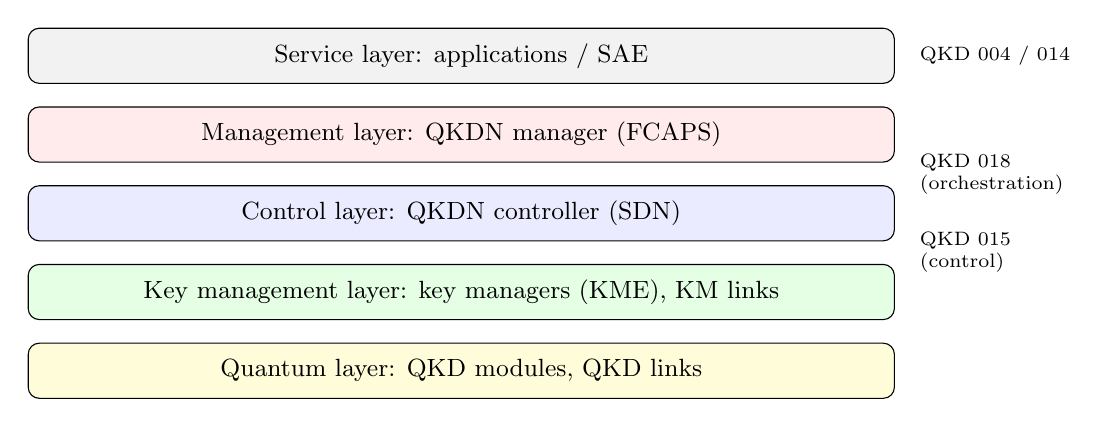
\begin{tikzpicture}[
  layer/.style={draw,rounded corners,minimum width=11cm,minimum height=7mm,
                align=center,font=\small},
  side/.style={font=\scriptsize,align=left,anchor=west}]
  \node[layer,fill=gray!10]   (srv) at (0,0)    {Service layer: applications / SAE};
  \node[layer,fill=red!8]     (mgm) at (0,-1.0) {Management layer: QKDN manager (FCAPS)};
  \node[layer,fill=blue!8]    (ctl) at (0,-2.0) {Control layer: QKDN controller (SDN)};
  \node[layer,fill=green!10]  (km)  at (0,-3.0) {Key management layer: key managers (KME), KM links};
  \node[layer,fill=yellow!15] (q)   at (0,-4.0) {Quantum layer: QKD modules, QKD links};
  \node[side] at (5.7,0)    {QKD 004 / 014};
  \node[side] at (5.7,-1.5) {QKD 018\\(orchestration)};
  \node[side] at (5.7,-2.5) {QKD 015\\(control)};
\end{tikzpicture}
\caption{Layered architecture of a QKD network according to ITU-T
Y.3800~\cite{ituy3800}; on the right, the indicative position of the ETSI
specifications discussed in the text.}
\label{fig:itu}
\end{figure}


Applications do not see the quantum part. A \emph{Secure Application
Entity} (SAE) requests keys from the \emph{Key Management Entity} (KME) of
its node through the GS~QKD~004~\cite{qkd004} or GS~QKD~014~\cite{qkd014}
APIs; two SAEs that want to communicate obtain the same key from their
respective KMEs, identified by a \emph{key ID}.

\paragraph{Software-Defined Networking.}
In a traditional network each device decides on its own how to forward
traffic. SDN~\cite{kreutz2015} instead separates three planes: the
\emph{data plane}, made of devices that execute; the \emph{control plane},
centralised in a controller with a global view of the network; and the
\emph{management and application plane}, which expresses goals. The
controller talks to the devices through a \emph{southbound} interface (SBI)
and offers its services upwards through a \emph{northbound} interface
(NBI). When there is more than one domain, an \emph{orchestrator} is added
above the controllers to coordinate end-to-end services without knowing
the details of each domain.

A QKD network has every feature that makes SDN useful: scarce and variable
resources (the key), tight physical constraints (attenuation, coexistence
with classical channels), multi-vendor equipment and demand that changes
over time. The two specifications that follow describe why and how ETSI
applied this paradigm to QKD.
